\documentclass[11pt,a4paper]{article}
\usepackage[T1]{fontenc}
\usepackage[utf8]{inputenc}
\usepackage{lmodern,microtype}
\usepackage[margin=25mm]{geometry}
\usepackage{amsmath,amssymb,amsthm,mathtools}
\usepackage{booktabs,array,longtable,graphicx,xcolor}
\usepackage{enumitem,fancyhdr,listings}
\usepackage[colorlinks=true,linkcolor=teal!65!black,urlcolor=teal!65!black,citecolor=teal!65!black]{hyperref}
\usepackage[nameinlink,noabbrev]{cleveref}
\definecolor{ink}{HTML}{173640}
\definecolor{teal}{HTML}{0F766E}
\definecolor{rust}{HTML}{B65C2D}
\pagestyle{fancy}\fancyhf{}
\fancyhead[L]{\small Extreme orthographic shadows}
\fancyhead[R]{\small Exact geometry and iPRA}
\fancyfoot[C]{\thepage}
\setlength{\headheight}{14pt}
\setlength{\parskip}{4pt}
\setlength{\parindent}{0pt}
\setlist{nosep,topsep=4pt,leftmargin=1.5em}
\newtheorem{theorem}{Theorem}[section]
\newtheorem{lemma}[theorem]{Lemma}
\newtheorem{proposition}[theorem]{Proposition}
\newtheorem{definition}[theorem]{Definition}
\newtheorem{remark}[theorem]{Remark}
\newcommand{\ph}{\varphi}
\newcommand{\rr}{\rho}
\newcommand{\Q}{\mathbb Q}
\newcommand{\R}{\mathbb R}
\newcommand{\N}{\mathbb N}
\newcommand{\Z}{\mathbb Z}
\newcommand{\ipra}{\mathrm{iPRA}}
\newcommand{\norm}[1]{\left\lVert#1\right\rVert}
\newcommand{\abs}[1]{\left|#1\right|}
\newcommand{\conv}{\operatorname{conv}}
\newcommand{\sgn}{\operatorname{sgn}}
\newcommand{\area}{\operatorname{area}}
\newcommand{\diag}{\operatorname{diag}}
\newcommand{\code}[1]{\texttt{#1}}
\lstset{basicstyle=\ttfamily\footnotesize,breaklines=true,columns=fullflexible,
 frame=single,rulecolor=\color{black!15},backgroundcolor=\color{black!2},showstringspaces=false}
\hypersetup{pdftitle={Extreme Orthographic Shadows of the Five Platonic Solids},
pdfauthor={Research report prepared for Vladimir Reshetnikov}}

\begin{document}
\hypersetup{pageanchor=false}
\begin{titlepage}
\vspace*{16mm}
{\color{teal}\large EXACT GEOMETRY \quad / \quad CONSTRUCTIVE ARITHMETIC\par}
\vspace{9mm}
{\color{ink}\Huge\bfseries Extreme Orthographic Shadows\\[4mm]of the Five Platonic Solids\par}
\vspace{9mm}
{\Large Largest and smallest projection areas, explicit orientations, and finite proofs in intuitionistic primitive recursive arithmetic\par}
\vspace{10mm}
{\large Prepared for Vladimir Reshetnikov\\19 November 2026\par}
\vspace{12mm}
\textbf{Main result.} All ten extrema are explicit algebraic multiples of the square of the edge length. The minimum for the icosahedron occurs away from its usual rotational symmetry axes. The other extremizing orientations have familiar geometric descriptions.

\textbf{Method.} A finite face-area formula converts projection area into a sum of absolute linear forms. Upper bounds follow from signed sums; lower bounds follow from an explicit two-stage decomposition into cross-product directions. All deciding arithmetic takes place in $\Q(\ph)$, where $\ph=(1+\sqrt5)/2$.

\textbf{Deliverable status.} The human argument is complete, and the accompanying exact-arithmetic programs were run successfully. The Lean file is an explicitly uncompiled formalization outline. It does not claim to contain a completed kernel-checked derivation of the new theorem. The distinction between an arithmetic theorem of iPRA and its real-geometric interpretation is developed in Sections~\ref{sec:ipra}--\ref{sec:lean}.
\vfill
{\small Includes exact certificate data, a dependency-free verifier, reproducible figures, a Lean outline, and pinned ProveIt source references.}
\end{titlepage}
\hypersetup{pageanchor=true}

\tableofcontents
\newpage

\section{The answers and what an orientation means}\label{sec:answers}

Fix an edge length $a>0$. A viewing direction is a nonzero vector $v$; the screen is a plane perpendicular to $v$. Translation of the screen and rotation within the screen do not affect area. We may put the center of the solid at the origin, use the screen
\[
 S_v=\{X:v\cdot X=0\},\qquad
 \pi_v(X)=X-\frac{v\cdot X}{v\cdot v}\,v,
\]
and write $u=v/\norm v$ when a unit direction is convenient. The two directions $v$ and $-v$ give the same shadow. All areas scale as $a^2$.

\begin{theorem}[All ten extrema]\label{thm:answers}
The minimum and maximum areas of orthogonal projections of regular Platonic solids of edge length $a$ are as follows.
\begin{center}
\renewcommand{\arraystretch}{1.65}
\begin{tabular}{@{}lcc@{}}
\toprule
Solid & Minimum area divided by $a^2$ & Maximum area divided by $a^2$\\
\midrule
Tetrahedron & $\dfrac1{2\sqrt2}$ & $\dfrac12$\\
Cube & $1$ & $\sqrt3$\\
Octahedron & $\dfrac1{\sqrt2}$ & $1$\\
Dodecahedron & $\dfrac{5+2\sqrt5}{2}$ & $\dfrac{\sqrt{250+110\sqrt5}}4$\\
Icosahedron & $\dfrac{\sqrt{35+15\sqrt5}}4$ & $\dfrac{\sqrt3(3+\sqrt5)}4$\\
\bottomrule
\end{tabular}
\end{center}
Each bound is attained by the orientations specified below.
\end{theorem}

\begin{center}
\small\renewcommand{\arraystretch}{1.35}
\begin{tabular}{@{}lp{58mm}p{58mm}@{}}
\toprule
Solid & A minimum orientation and shadow & A maximum orientation and shadow\\
\midrule
Tetrahedron & View parallel to an edge: an isosceles triangle. & View along the line joining midpoints of opposite edges: a square.\\
Cube & View normally to a face: a square. & View along a body diagonal: a regular hexagon.\\
Octahedron & View through opposite edge midpoints: a rhombus. & View through opposite vertices: a square.\\
Dodecahedron & View through opposite edge midpoints: a centrally symmetric hexagon. & View normally to a face: a regular decagon.\\
Icosahedron & View along $(1,1,0)$ in \eqref{eq:icovertices}: a centrally symmetric hexagon. & View normally to a face: a regular hexagon.\\
\bottomrule
\end{tabular}
\end{center}

For unit edge length the pairs of areas are, respectively,
\[
\begin{array}{c|cc}
 &\text{minimum}&\text{maximum}\\\hline
\text{tetrahedron}&0.353553391&0.500000000\\
\text{cube}&1.000000000&1.732050808\\
\text{octahedron}&0.707106781&1.000000000\\
\text{dodecahedron}&4.736067977&5.567581822\\
\text{icosahedron}&2.069737599&2.267283942
\end{array}
\]
These decimals are for convenience; none is used in a proof.

The unusual icosahedral orientation is completely concrete. In the coordinates specified below, two nonadjacent faces have normal directions $(1,-1,1)$ and $(1,-1,-1)$. The viewing line $(1,1,0)$ is parallel to both face planes. Those faces and their opposites are seen edge-on. Checking only face, vertex, and edge-midpoint axes would miss this minimum.

\section{Coordinate models and a finite projection formula}\label{sec:geometry}

\subsection{Coordinates and scaling}
Put
\[
 \ph=\frac{1+\sqrt5}{2},\qquad \rr=\ph-1=\ph^{-1},\qquad
 \ph^2=\ph+1,\quad \rr^2=2-\ph.
\]
Signs in a displayed coordinate family are independent. The solids are the convex hulls of the following vertices:
\begin{align}
 V_T&=\frac{a}{2\sqrt2}\{(1,1,1),(1,-1,-1),(-1,1,-1),(-1,-1,1)\},\label{eq:tetvertices}\\
 V_C&=\frac a2\{(\pm1,\pm1,\pm1)\},\label{eq:cubevertices}\\
 V_O&=\frac a{\sqrt2}\{\pm e_1,\pm e_2,\pm e_3\},\label{eq:octvertices}\\
 V_D&=\frac{a\ph}{2}\{(\pm1,\pm1,\pm1),(0,\pm\ph,\pm\rr),
 (\pm\rr,0,\pm\ph),(\pm\ph,\pm\rr,0)\},\label{eq:dodecvertices}\\
 V_I&=\frac a2\{(0,\pm\ph,\pm1),(\pm\ph,\pm1,0),(\pm1,0,\pm\ph)\}.
 \label{eq:icovertices}
\end{align}
Here $e_1,e_2,e_3$ are the coordinate unit vectors. The raw edge squares, before the displayed scalings, are $8,4,2,4\rr^2,4$, respectively.

These descriptions can be verified finitely. All vertices of each model have the same squared distance from the origin. Supporting planes give triangular faces for $T,O,I$, squares for $C$, and pentagons for $D$. For a dodecahedral example, the raw face $x+\ph y=\ph^2$ has cyclic vertices
\[
 (\ph,\rr,0),\ (1,1,1),\ (0,\ph,\rr),\ (0,\ph,-\rr),\ (1,1,-1).
\]
Its consecutive squared distances are $4\rr^2$ and its diagonal squares are $4$; thus each diagonal is $\ph$ times a side. The five vertices are on a circle in their supporting plane and form a convex regular pentagon. For the icosahedron, the raw face with normal $(1,1,1)$ consists of $(0,\ph,1),(\ph,1,0),(1,0,\ph)$, with all side lengths $2$.

The verifier in the archive independently enumerates all supporting triples of vertices, identifies all facets, orders their edges, checks the regular-face distance identities, and calculates their area vectors. There are at most $\binom{20}{3}=1140$ supporting-triple tests. This supplements the displayed coordinate argument with a complete finite certificate, including degenerate supporting triples.

\subsection{Area vectors and the shadow identity}
For a face with vertices $p_0,\ldots,p_{r-1}$ in outward cyclic order, define its area vector by
\begin{equation}
 W_F=\frac12\sum_{j=0}^{r-1}p_j\times p_{j+1},\qquad p_r=p_0.
 \label{eq:areavector}
\end{equation}
Translation invariance follows by telescoping. A triangle has area vector
$\frac12(p_1-p_0)\times(p_2-p_0)$; a fan triangulation proves
$W_F=\area(F)n_F$, with $n_F$ the outward unit normal.

\begin{lemma}[Finite polyhedral brightness formula]\label{lem:brightness}
For a convex polyhedron $P$ and $v\ne0$,
\begin{equation}
 \area(\pi_vP)=\frac1{2\norm v}\sum_F\abs{W_F\cdot v}.
 \label{eq:cauchy}
\end{equation}
\end{lemma}
\begin{proof}
Orthogonal projection of a face has area $\abs{W_F\cdot v}/\norm v$; this follows first for a triangle by the cross-product determinant identity, then for a face by triangulation.

Consider a line parallel to $v$ above an interior point of the shadow. Its intersection with the solid is a nondegenerate interval, except on projected boundary pieces. Outside the finite union of projected edges, its upper and lower endpoints lie in unique relative interiors of faces. The upper face has $W_F\cdot v>0$, and the lower face has $W_F\cdot v<0$. The projected positive faces therefore dissect the shadow once, and the projected negative faces dissect it a second time. Faces with $W_F\cdot v=0$ project to line segments and contribute zero area. Summing the two dissections proves \eqref{eq:cauchy}.

This is finite polygonal area reasoning, not an integration argument. To make the treatment of boundaries literal, refine the screen by all projected edge lines and triangulate the resulting cells. Membership in each projected face is constant on each open cell. The endpoint argument gives multiplicity two on every two-dimensional cell; segments and points have determinant area zero.

For arithmetic coordinates, one need not construct an orthonormal screen basis. Choose a coordinate $j$ with $v_j\ne0$ and project along $v$ onto the coordinate plane $X_j=0$ by
\[
 q(X)=X-\frac{X_j}{v_j}v.
\]
This uses only field operations. Orthogonal projection from that coordinate plane onto $S_v$ multiplies area by $\abs{v_j}/\norm v$. Consequently all dissection checks can be performed with two-dimensional determinants in the original field; the single factor $\norm v$ is left outside.
\end{proof}

\subsection{The five absolute-linear functions}\label{sec:generators}
Let
\[
 T=\{(1,1,1),(1,-1,-1),(-1,1,-1),(-1,-1,1)\},
\]
and define the following representative lists:
\begin{align*}
 G_C={}&(e_1,e_2,e_3),\qquad G_T=G_O=T,\\
 G_D={}&((0,1,\ph),(0,1,-\ph),(1,\ph,0),(1,-\ph,0),(\ph,0,1),(\ph,0,-1)),\\
 G_I={}&(g_1,\ldots,g_{10}),
\end{align*}
where
\begin{equation}\label{eq:icolonormals}
\begin{array}{llll}
g_1=(1,1,1),&g_2=(1,1,-1),&g_3=(1,-1,1),&g_4=(-1,1,1),\\
g_5=(0,\rr,\ph),&g_6=(0,\rr,-\ph),&g_7=(\rr,\ph,0),&g_8=(\rr,-\ph,0),\\
g_9=(\ph,0,\rr),&g_{10}=(\ph,0,-\rr).
\end{array}
\end{equation}
For any list $G=(g_i)$ write
\[
 F_G(v)=\sum_i\abs{g_i\cdot v},\qquad Q(v)=v\cdot v.
\]
Direct use of \eqref{eq:areavector}--\eqref{eq:cauchy} gives
\begin{equation}\label{eq:area-factor}
 \area(\pi_v P)=a^2c_P\frac{F_{G_P}(v)}{\sqrt{Q(v)}},\qquad
 \begin{array}{c|ccccc}
 P&T&C&O&D&I\\\hline
 c_P&1/8&1&1/4&(\ph+2)/4&1/4.
 \end{array}
\end{equation}
For clarity, the unit-edge face area vectors are $-t/4$ for $t\in T$ in the tetrahedron; $\pm e_i$ for the cube; all eight sign vectors divided by $4$ for the octahedron; $\pm(\ph+2)g/4$ for $g\in G_D$; and $\pm g/4$ for $g\in G_I$. Opposite faces combine into one absolute term. The tetrahedron uses all four faces and retains the factor $1/2$ from \eqref{eq:cauchy}.

For the dodecahedral example above, the raw face area vector is $(3-\ph)(1,\ph,0)$. Multiplying by the squared scale $a^2\ph^2/4$ gives $a^2(\ph+2)(1,\ph,0)/4$. Thus no pentagonal trigonometric formula is needed. Its face area, if desired, is $a^2\sqrt{25+10\sqrt5}/4$.

\section{A finite algebraic extremum theorem}\label{sec:finite}

The next result is the central constructive tool. It will be proved over the ordered field $K=\Q(\ph)$, where signs are decidable; Section~\ref{sec:ipra} gives its arithmetical implementation. Ordinary real-geometric consequences follow with an explicit continuity bound, without deciding signs of arbitrary constructive reals.

\begin{theorem}[Signed sums and cross products]\label{thm:finite}
Let $g_1,\ldots,g_m\in K^3$ span three-space, and put $F(x)=\sum_i\abs{g_i\cdot x}$. Suppose $L,U\ge0$ and the following finite checks hold:
\begin{align}
 Q\!\left(\sum_i\epsilon_i g_i\right)&\le U
 &&\text{for every }\epsilon\in\{-1,1\}^m,\label{eq:uppercert}\\
 LQ(g_i\times g_j)&\le F(g_i\times g_j)^2
 &&\text{for every }i<j\text{ with }g_i\times g_j\ne0.\label{eq:lowercert}
\end{align}
Then every $x\in K^3$ satisfies
\begin{equation}\label{eq:universal}
 LQ(x)\le F(x)^2\le UQ(x).
\end{equation}
An explicitly supplied nonzero vector satisfying equality certifies attainment of the corresponding bound.
\end{theorem}

\subsection{Proof of the upper bound}
Choose $\epsilon_i$ to be $1$ when $g_i\cdot x\ge0$ and $-1$ otherwise, and set $s=\sum_i\epsilon_i g_i$. Then $F(x)=s\cdot x$. Lagrange's identity gives
\[
 Q(s)Q(x)-(s\cdot x)^2=Q(s\times x)\ge0.
\]
Together with \eqref{eq:uppercert}, this proves the upper inequality. Moreover, a signed sum $s$ with $Q(s)=U>0$ itself yields an attaining direction: $F(s)\ge s\cdot s=U$, while the upper bound gives $F(s)^2\le U^2$. Alternatively, attainment can be checked directly at a simpler direction.

\subsection{Proof of the lower bound: a bounded construction}
The case $x=0$ is immediate. Otherwise spanning implies $F(x)>0$. Select signs as above, put $w_i=\epsilon_i g_i$ and $\ell=\sum_iw_i$, and consider
\[
 C=\{y:w_i\cdot y\ge0\ (1\le i\le m)\},\qquad
 p=\frac{x}{F(x)}.
\]
On $C$ the function $F$ is exactly $\ell\cdot y$, so $p\in C$ and $\ell\cdot p=1$.

A constraint is \emph{active} at $p$ if $w_i\cdot p=0$. Its active normals have rank at most two, since three independent active normals would force $p=0$. If two independent normals are active, the point is parallel to their cross product and we stop. Otherwise we split it as follows.

If one independent normal $w_j$ is active, choose $d=\ell\times w_j$. It is nonzero: proportionality of $\ell$ and $w_j$ would contradict their values $1$ and $0$ on $p$. Every active normal is proportional to $w_j$, so $d$ preserves all active constraints. If the active normals have rank zero, choose the first basis vector $e_j$ with $\ell\times e_j\ne0$ and put $d=\ell\times e_j$. Such a basis vector exists because $\ell\cdot p=1$; any active zero normals are automatically preserved. In either case,
\[
 d\ne0,\qquad \ell\cdot d=0,\qquad w_i\cdot d=0\text{ at every active index}.
\]
Write $a_i=w_i\cdot p$ and $b_i=w_i\cdot d$. The $b_i$ sum to zero, and they are not all zero because the $w_i$ span. Thus both positive and negative values occur. Whenever $b_i\ne0$, the corresponding $a_i$ is strictly positive. The following finite, nonempty minima therefore exist and are positive:
\[
 t_+=\min_{b_i<0}\frac{a_i}{-b_i},\qquad
 t_-=\min_{b_i>0}\frac{a_i}{b_i}.
\]
Set $p_+=p+t_+d$ and $p_-=p-t_-d$. Both remain in $C$ and in the slice $\ell\cdot y=1$. Each gains an active normal independent of the old active normals, since a dependent normal would have zero slope along $d$. Furthermore,
\begin{equation}\label{eq:split}
 p=\frac{t_-}{t_++t_-}p_++\frac{t_+}{t_++t_-}p_-.
\end{equation}
Thus active rank increases on each branch. At most two splitting levels, or three splitting calls in total, produce at most four terminal points $z_\alpha$ with explicitly computed nonnegative weights $\theta_\alpha$ summing to one.

At a terminal point two independent normals are active. For an appropriate sign of their cross product $r$, the terminal point equals $r/F(r)$. Consequently \eqref{eq:lowercert} gives $LQ(z_\alpha)\le1$. Finally, the exact polynomial identity
\begin{equation}\label{eq:convexsquare}
 \sum_\alpha\theta_\alpha Q(z_\alpha)
 -Q\!\left(\sum_\alpha\theta_\alpha z_\alpha\right)
 =\sum_{\alpha<\beta}\theta_\alpha\theta_\beta Q(z_\alpha-z_\beta)\ge0
\end{equation}
shows that $LQ(p)\le1$. Multiplying by $F(x)^2$ proves the lower inequality in \eqref{eq:universal}.

All divisions used above have explicitly positive or nonzero denominators. Each minimum is a scan of at most $m$ rational-field numbers; no search is waiting for an unspecified event to happen. There is no compactness or least-value principle in the argument.

\subsection{The complete finite data for this problem}
For the generator lists in Section~\ref{sec:generators}, spanning can be certified by one nonzero triple determinant. The exact table is:
\begin{center}
\renewcommand{\arraystretch}{1.25}
\begin{tabular}{@{}lrrrrr@{}}
\toprule
Solid & $m$ & signed sums & cross pairs & $L$ & $U$\\
\midrule
Tetrahedron &4&16&6&$8$&$16$\\
Cube &3&8&3&$1$&$3$\\
Octahedron &4&16&6&$8$&$16$\\
Dodecahedron &6&64&15&$8+12\ph$&$12+16\ph$\\
Icosahedron &10&1024&45&$20+30\ph$&$24+36\ph$\\
\bottomrule
\end{tabular}
\end{center}
The remaining sections prove these values by smaller hand-verifiable calculations and supply explicit attaining directions and shadows. The archive also contains every row of the larger, uniform certificate.

\section{The tetrahedron, cube, and octahedron}\label{sec:simple}

\subsection{The cube}
Put $x=\abs{u_1}$, $y=\abs{u_2}$, $z=\abs{u_3}$, where $u$ is unit. Formula~\eqref{eq:area-factor} becomes
\[
 A_C(u)=a^2(x+y+z).
\]
The two exact identities
\[
 (x+y+z)^2-(x^2+y^2+z^2)=2(xy+yz+zx)\ge0,
\]
\[
 3(x^2+y^2+z^2)-(x+y+z)^2=(x-y)^2+(y-z)^2+(z-x)^2\ge0
\]
prove $a^2\le A_C(u)\le\sqrt3a^2$. The first equality is attained at $u=e_1$ and the second at $u=(1,1,1)/\sqrt3$.

In the first direction the shadow is a square of side $a$. In the second it is a regular hexagon: six projected vertices are extreme and the two vertices on the viewing diagonal project to the center. Its side length and circumradius are $a\sqrt{2/3}$, giving area $\sqrt3a^2$.

\subsection{One common function for the tetrahedron and octahedron}
Put $x=\abs{u_1}$, $y=\abs{u_2}$, $z=\abs{u_3}$, and set $s=x+y+z$, $M=\max(x,y,z)$ and
\[
 h=\max(M,s/2).
\]
Pairing signs in $T$ gives the elementary identity
\begin{equation}\label{eq:fourabs}
 F_T(u)=\abs{x+y+z}+\abs{x+y-z}+\abs{x-y+z}+\abs{-x+y+z}
 =\max(4M,2s)=4h.
\end{equation}
To verify it, if one coordinate is at least the sum of the other two, the expression is four times that coordinate; otherwise all three triangle differences are nonnegative and the expression is $2s$.

Since each coordinate is at most $h$ and their sum is at most $2h$,
\begin{equation}\label{eq:smalllower}
 x^2+y^2+z^2\le h(x+y+z)\le2h^2.
\end{equation}
Conversely $M^2\le Q(u)$ and $s^2\le3Q(u)\le4Q(u)$, so $h^2\le Q(u)$. Therefore
\[
 8Q(u)\le F_T(u)^2\le16Q(u).
\]
This proof uses only sums, products, order, and a finite maximum. Lower equality is attained at $(1,1,0)$; upper equality at $e_1$.

For the tetrahedron the multiplier is $a^2/8$. Thus
\[
 A_{T,\min}=\frac{a^2}{2\sqrt2},\qquad A_{T,\max}=\frac{a^2}{2}.
\]
The direction $(1,1,0)$ is parallel to the edge joining $(1,1,1)$ and $(-1,-1,1)$ in \eqref{eq:tetvertices}. In screen coordinates along $(1,-1,0)/\sqrt2$ and $e_3$, the shadow has vertices
\[
 \left(0,\frac{a}{2\sqrt2}\right),\qquad
 \left(\pm\frac a2,-\frac{a}{2\sqrt2}\right).
\]
It is an isosceles triangle of base $a$, height $a/\sqrt2$, and equal sides $\sqrt3a/2$. In direction $e_1$, the shadow is the square with screen vertices $(\pm a/(2\sqrt2),\pm a/(2\sqrt2))$. The viewing axis joins the midpoints of opposite edges.

For the octahedron the multiplier is $a^2/4$. Thus
\[
 A_{O,\min}=\frac{a^2}{\sqrt2},\qquad A_{O,\max}=a^2.
\]
In direction $(1,1,0)$, using the same screen basis, the extreme points are
\[
 (\pm a/2,0),\qquad(0,\pm a/\sqrt2).
\]
This rhombus has diagonals $a$ and $\sqrt2a$, and side length $\sqrt3a/2$. The viewing line joins opposite edge midpoints. In direction $e_1$, the shadow has vertices $(\pm a/\sqrt2,0),(0,\pm a/\sqrt2)$, a square of side $a$ viewed along a vertex-to-vertex axis.

\section{The dodecahedron}\label{sec:dodeca}

\subsection{A sum of three maxima}
For $x,y,z\ge0$ the identity $\abs{b+c}+\abs{b-c}=2\max(\abs b,\abs c)$ reduces the six normal terms to
\begin{equation}\label{eq:dodecG}
 F_{G_D}(u)=2G(x,y,z),\qquad
 G=\max(y,\ph z)+\max(x,\ph y)+\max(\ph x,z).
\end{equation}
Consequently, for a unit direction,
\begin{equation}\label{eq:dodecarea}
 A_D(u)=\frac{a^2(\ph+2)}2G(x,y,z).
\end{equation}
The coordinate sign changes used here preserve the normal set, so absolute coordinates lose no orientations.

\subsection{Maximum: eight coefficient vectors}
Expand the three binary maxima in \eqref{eq:dodecG}. If a bit $0$ selects the first entry and $1$ the second, $G$ is the maximum of the eight linear forms $c\cdot(x,y,z)$ in this table:
\begin{center}
\renewcommand{\arraystretch}{1.2}
\begin{tabular}{@{}ccc@{}}\toprule
Bits & $c$ & $Q(c)$\\\midrule
000&$(\ph^2,1,0)$&$3\ph^2$\\
001&$(1,1,1)$&$3$\\
010&$(\ph,\ph^2,0)$&$4\ph+3$\\
011&$(0,\ph^2,1)$&$3\ph^2$\\
100&$(\ph^2,0,\ph)$&$4\ph+3$\\
101&$(1,0,\ph^2)$&$3\ph^2$\\
110&$(\ph,\ph,\ph)$&$3\ph^2$\\
111&$(0,\ph,\ph^2)$&$4\ph+3$\\\bottomrule
\end{tabular}
\end{center}
Each entry follows from $\ph^2=\ph+1$. Since $4\ph+3>3\ph^2>3$, Lagrange's identity proves $G(v)^2\le(4\ph+3)Q(v)$. Equality occurs in the direction $(1,\ph,0)$: its coefficient vector $(\ph,\ph^2,0)$ is parallel to that direction. Therefore
\[
 A_{D,\max}=\frac{a^2(\ph+2)}2\sqrt{4\ph+3}
 =\frac{a^2}4\sqrt{250+110\sqrt5}.
\]
The direction is a face normal; the screen is parallel to that face.

\subsection{Minimum: an explicit small cone proof}
We prove
\begin{equation}\label{eq:dodeclower}
 G(v)^2\ge\ph^4Q(v)\qquad(v\in K_{\ge0}^3).
\end{equation}
Define
\[
 E_i=e_i,\quad T_1=(\ph,1,0),\ T_2=(0,\ph,1),\ T_3=(1,0,\ph),
\]
\[
 P=(\ph^2,\ph,1),\quad Q_0=(1,\ph^2,\ph),\quad S=(\ph,1,\ph^2).
\]
The symbol $Q_0$ names a ray and should not be confused with the squared-norm function $Q$.
On the ray families,
\[
\begin{array}{c|cc}
 r&G(r)&Q(r)\\\hline
 E_i&\ph^2&1\\
 T_i&2\ph^2&\ph+2\\
 P,Q_0,S&2\ph^3&4\ph^2
\end{array}
\]
so \eqref{eq:dodeclower} holds on each ray; it is strict on $T_i$ because $\ph+2<4$.

The comparison planes $y=\ph z$, $x=\ph y$, $z=\ph x$ divide the positive octant into the following chambers, labeled by the selected bits as in the maximum table:
\begin{center}
\begin{tabular}{@{}clcl@{}}\toprule
Bits&Generating rays&Bits&Generating rays\\\midrule
000&$E_1,T_1,P$&001&no nonzero point\\
010&$E_2,T_1,P,Q_0$&011&$E_2,T_2,Q_0$\\
100&$E_1,T_3,P,S$&101&$E_3,T_3,S$\\
110&$P,Q_0,S$&111&$E_3,T_2,Q_0,S$\\\bottomrule
\end{tabular}
\end{center}
Here closed chambers may overlap on their boundary. The allegedly missing chamber would require $y\ge\ph z$, $x\ge\ph y$, $z\ge\ph x$, forcing $x=y=z=0$ because $\ph^3>1$.

For completeness, the following formulas prove the entire covering by nonnegative combinations. Cyclic coordinate permutation handles chambers of the same type.

In chamber 000,
\[
 (x,y,z)=(x-\ph y)E_1+(y-\ph z)T_1+zP.
\]
In chamber 010, the inequalities are $y\ge\ph z$, $x\le\ph y$, $z\le\ph x$. If $x\ge\ph^2z$, use
\[
 (x,y,z)=(y-x/\ph)E_2+(x/\ph-\ph z)T_1+zP.
\]
If $x\le\ph^2z$, use
\[
 (x,y,z)=(y-\ph z)E_2+\frac{\ph x-z}{2\ph}P
                   +\frac{\ph^2z-x}{2\ph}Q_0.
\]
In chamber 110, use
\[
 (x,y,z)=\frac{\ph x-z}{2\ph}P+\frac{\ph y-x}{2\ph}Q_0
                         +\frac{\ph z-y}{2\ph}S.
\]
All coefficients are nonnegative by the chamber inequalities, and direct multiplication verifies every identity.

There is also a purely polynomial way to propagate the ray bounds. On one chamber $G$ is linear. If $v=\sum_{i=1}^3\lambda_ir_i$, then
\[
 G(v)^2-\ph^4Q(v)=\lambda^{\mathsf T}M\lambda,
 \qquad M_{ij}=G(r_i)G(r_j)-\ph^4(r_i\cdot r_j).
\]
For the four ordered ray triples appearing above, the respective matrices are
\[
\begin{array}{c@{\qquad}c}
\left(\begin{smallmatrix}0&\ph^2&\ph^3\\\ph^2&\ph^2&\ph^3\\\ph^3&\ph^3&0\end{smallmatrix}\right)&
\left(\begin{smallmatrix}0&\ph^4&\ph^5\\\ph^4&\ph^2&\ph^3\\\ph^5&\ph^3&0\end{smallmatrix}\right)\\[3mm]
\left(\begin{smallmatrix}0&\ph^5&\ph^3\\\ph^5&0&2\ph^4\\\ph^3&2\ph^4&0\end{smallmatrix}\right)&
\left(\begin{smallmatrix}0&2\ph^4&2\ph^4\\2\ph^4&0&2\ph^4\\2\ph^4&2\ph^4&0\end{smallmatrix}\right).
\end{array}
\]
Their order is $(E_1,T_1,P)$, $(E_2,T_1,P)$, $(E_2,P,Q_0)$, $(P,Q_0,S)$. Every entry is nonnegative. This proves \eqref{eq:dodeclower} in all chambers without square roots or a triangle-inequality theorem.

At $v=e_1$, $G(v)=\ph^2$. Hence
\[
 A_{D,\min}=\frac{a^2(\ph+2)\ph^2}{2}
            =\frac{5+2\sqrt5}{2}\,a^2.
\]
The raw vertices $(\ph,\rr,0)$ and $(\ph,-\rr,0)$ are adjacent and have midpoint on the $e_1$ axis, verifying its edge-midpoint description. The other algebraic attaining rays in the table are related by the solid's symmetries.

\subsection{The two shadows}
For the minimum direction $e_1$, use screen coordinates $(y,z)$. In cyclic order the six vertices are
\begin{equation}\label{eq:dodechex}
 \frac{a\ph}{2}\bigl((0,\ph),(\ph,\rr),(\ph,-\rr),
              (0,-\ph),(-\ph,-\rr),(-\ph,\rr)\bigr).
\end{equation}
The projected points $(\pm1,\pm1)$ lie on its sloping sides before scaling; for instance the upper-right side has equation $z=\ph-y/\ph$. All other projected vertices lie inside. The raw area is $4+2\ph$, giving the minimum after multiplication by $a^2\ph^2/4$.

For the maximum put $R=\sqrt{\ph+2}$ and use unit normal $(1,\ph,0)/R$. An orthonormal screen coordinate system is
\[
 (s,t)=\left(z,\frac{\ph x-y}{R}\right).
\]
Before the scale $a\ph/2$, its ten cyclic extreme vertices are
\begin{align*}
 &(0,2\ph/R),\ (-1,\ph^2/R),\ (-\ph,1/R),\ (-\ph,-1/R),\ (-1,-\ph^2/R),\\
 &(0,-2\ph/R),\ (1,-\ph^2/R),\ (\ph,-1/R),\ (\ph,1/R),\ (1,\ph^2/R).
\end{align*}
Each has radius $2\ph/R$ and consecutive distances $2/R$. The other projected vertices satisfy the ten edge half-plane inequalities. Thus the shadow is a regular decagon, with side $a\ph/R$ and circumradius $a\ph^2/R$.

\section{The icosahedron}\label{sec:ico}

\subsection{Maximum: a 32-vector calculation}
Use the normal list \eqref{eq:icolonormals}. Coordinate sign changes preserve the full set of normal lines, so again put $x=\abs{u_1}$, $y=\abs{u_2}$, $z=\abs{u_3}$. Equations \eqref{eq:fourabs} and the paired-absolute-value identity give $F_{G_I}=2H$, where
\begin{equation}\label{eq:icoH}
 H=\max(x+y+z,2x,2y,2z)
  +\max(\rr x,\ph y)+\max(\rr y,\ph z)+\max(\ph x,\rr z).
\end{equation}
Thus $H$ is the maximum of 32 linear forms with coefficient vectors
\[
 c=b+p_0+p_1+p_2,
\]
where
\begin{align*}
 b&\in\{(1,1,1),(2,0,0),(0,2,0),(0,0,2)\},\\
 p_0&\in\{(\rr,0,0),(0,\ph,0)\},\quad
 p_1\in\{(0,\rr,0),(0,0,\ph)\},\quad
 p_2\in\{(\ph,0,0),(0,0,\rr)\}.
\end{align*}
Write bits $0,1$ for the first and second choices in each pair. The squared coefficient norms are shown below. The two omitted choices of $b$ have the same multiset as $b=(2,0,0)$, by cyclic coordinate permutation.
\begin{center}
\small\setlength{\tabcolsep}{4pt}\renewcommand{\arraystretch}{1.3}
\begin{tabular}{@{}c*{4}{c}@{}}\toprule
$b$&000&001&010&011\\\midrule
$(1,1,1)$&$6+5\ph$&$3+3\ph$&$7+7\ph$&$6+5\ph$\\
$(2,0,0)$&$7+7\ph$&$6+\ph$&$6+9\ph$&$7+3\ph$\\\midrule
$b$&100&101&110&111\\\midrule
$(1,1,1)$&$7+7\ph$&$6+5\ph$&$6+9\ph$&$7+7\ph$\\
$(2,0,0)$&$10+5\ph$&$11-\ph$&$7+7\ph$&$10+\ph$\\\bottomrule
\end{tabular}
\end{center}
Every entry is at most $6+9\ph=3\ph^4$. For example the differences from $7+7\ph$ and $10+5\ph$ are $2\ph-1$ and $4(\ph-1)$, both positive. The remaining comparisons follow at once from $1<\ph<2$. Lagrange's identity gives
\[
 H(v)^2\le3\ph^4Q(v),\qquad F_{G_I}(v)^2\le12\ph^4Q(v).
\]
The choice $b=(1,1,1)$ and bits 110 gives $c=\ph^2(1,1,1)$, proving attainment at $u=(1,1,1)/\sqrt3$. Hence
\[
 A_{I,\max}=\frac{a^2\sqrt3\ph^2}{2}
 =\frac{a^2\sqrt3(3+\sqrt5)}4.
\]
The viewing direction is normal to the explicit triangular face in Section~\ref{sec:geometry}.

\subsection{Minimum: all 45 candidate cross products}
The ten representatives span three-space: $g_1,g_2,g_3$ have nonzero determinant. Each has squared norm $3$. The complete cross-product calculation has just two types:
\begin{center}
\small\renewcommand{\arraystretch}{1.45}
\begin{tabular}{@{}crcccc@{}}\toprule
Type&Count&$\abs{g_i\cdot g_j}$&$Q(r_{ij})$&$F_{G_I}(r_{ij})$&$F_{G_I}(r_{ij})^2/Q(r_{ij})$\\\midrule
A&30&$1$&$8$&$10+6\sqrt5$&$35+15\sqrt5$\\
B&15&$\sqrt5$&$4$&$8+4\sqrt5$&$36+16\sqrt5$\\\bottomrule
\end{tabular}
\end{center}
Here $r_{ij}=g_i\times g_j$. To expose every case, the pair-type table is:
\begin{center}
\small\renewcommand{\arraystretch}{1.2}
\begin{tabular}{@{}c*{9}{c}@{}}\toprule
$i\backslash j$&2&3&4&5&6&7&8&9&10\\\midrule
1&A&A&A&B&A&B&A&B&A\\
2&&A&A&A&B&B&A&A&B\\
3&&&A&A&B&A&B&B&A\\
4&&&&B&A&A&B&A&B\\
5&&&&&B&A&A&A&A\\
6&&&&&&A&A&A&A\\
7&&&&&&&B&A&A\\
8&&&&&&&&A&A\\
9&&&&&&&&&B\\\bottomrule
\end{tabular}
\end{center}
This table is checked by taking each displayed cross product, then summing its ten absolute dot products. No group-theoretic classification is assumed. For illustration, $g_1\times g_2=(-2,2,0)$ and $F_{G_I}(1,1,0)=5+3\sqrt5$; coordinate sign invariance gives the same value at $(-1,1,0)$. Also
\[
 g_1\times g_5=(1,-\ph,\rr),\quad Q(g_1\times g_5)=4,
 \quad F_{G_I}(g_1\times g_5)=8+4\sqrt5.
\]
Every table entry is reducible using $\ph^2=\ph+1$ and exact sign comparisons; the independent integer-pair verifier in the archive reconstructs the full table.

Since $36+16\sqrt5-(35+15\sqrt5)=1+\sqrt5>0$, Theorem~\ref{thm:finite} gives
\[
 F_{G_I}(v)^2\ge(35+15\sqrt5)Q(v).
\]
At $v=(1,1,0)$, $Q(v)=2$ and $F_{G_I}(v)=5+3\sqrt5$. Therefore
\[
 A_{I,\min}=\frac{a^2(5+3\sqrt5)}{4\sqrt2}
 =\frac{a^2\sqrt{35+15\sqrt5}}4.
\]
This proves both the bound and its attainment, without an assumption that a minimum exists.

\subsection{The shadows and the minimum's orientation}
For $u=(1,1,0)/\sqrt2$, take the screen basis
\[
 e=\frac{(1,-1,0)}{\sqrt2},\qquad f=(0,0,1).
\]
The projected convex hull has six vertices
\begin{equation}\label{eq:icohex}
 \left(\pm\frac{a\ph^2}{2\sqrt2},0\right),\qquad
 \left(\pm\frac a{2\sqrt2},\pm\frac{a\ph}{2}\right).
\end{equation}
All four sign choices occur in the second family. Projecting the twelve original vertices verifies that the remaining points lie on or inside the six supporting sides. A central rectangle plus two triangles gives
\[
 \area=\frac{a^2\ph}{\sqrt2}+\frac{a^2\ph^2}{2\sqrt2}
       =\frac{a^2(3\ph+1)}{2\sqrt2},
\]
the value already proved. This is a centrally symmetric, nonregular hexagon.

The face-normal directions $(1,-1,1)$ and $(1,-1,-1)$ are both perpendicular to $u$. Their absolute dot product is $1$; these two faces share one vertex but no edge. In particular the direction is not a face axis. Inspection of \eqref{eq:icovertices} and of the finitely many edge midpoints also shows that $(1,1,0)$ is neither a vertex axis nor an edge-midpoint axis. This explains why the minimum is less obvious than a standard symmetry view.

For the maximum $u=(1,1,1)/\sqrt3$, six extreme projected vertices come from
\[
 \frac a2\{(-\ph,1,0),(-1,0,\ph),(0,-\ph,1),
             (\ph,-1,0),(1,0,-\ph),(0,\ph,-1)\}.
\]
They all have projected radius $a\ph/\sqrt3$. Central symmetry and the order-three rotation about the face axis give an order-six rotation on this set. The shadow is a regular hexagon of side $a\ph/\sqrt3$, and its area is $\sqrt3\ph^2a^2/2$.

\section{Precisely what is proved in iPRA}\label{sec:ipra}

\subsection{The theory and the numerical representations}
We use iPRA as first-order intuitionistic logic with equality, symbols and defining equations for primitive recursive functions, successor axioms, and induction for quantifier-free formulas. This is the convention documented in ProveIt \href{https://github.com/VladimirReshetnikov/ProveIt/blob/09fe17194da14cdd100947737952e44100bb71b8/Logic/PrimitiveRecursiveArithmetic/README.md}{(pinned README)}. We do not add a sort of arbitrary real numbers, unrestricted real trichotomy, or a theorem saying that a continuous function attains extrema.

Encode signed integers by a sign-and-magnitude or zigzag natural-number code. Encode a rational by a signed numerator and a positive denominator; equality is by cross multiplication, so lowest-term reduction is optional. Fixed tuples are encoded by a standard primitive recursive pairing. The elements of $K$ are \emph{pairs of rationals}
\[
 (b,c)\quad\text{representing }b+c\ph.
\]
They are not integers constrained by $\ph^2=\ph+1$, which would be a vacuous encoding. Field operations are
\begin{align*}
 (b,c)+(d,e)&=(b+d,c+e),\\
 (b,c)(d,e)&=(bd+ce,be+cd+ce),\\
 \overline{(b,c)}&=(b+c,-c),\\
 N(b,c)&=b^2+bc-c^2,\\
 (b,c)^{-1}&=((b+c)/N,-c/N)\qquad\text{if }(b,c)\ne(0,0).
\end{align*}
All code operations are totalized; a zero-denominator branch returns a fixed default, and the proof invariants show that such a branch is not used for an actual division in the argument.

For exact order, write
\[
 2(b+c\ph)=A+B\sqrt5,\qquad A=2b+c,\ B=c.
\]
If $A$ and $B$ have the same sign, that sign decides the result. If one is zero, the other decides. If they have opposite signs, compare $A^2$ with $5B^2$:
\[
 \sgn(A+B\sqrt5)=\sgn(A)\,\sgn(A^2-5B^2).
\]
These are rational comparisons, reducible to integer arithmetic.

For completeness, nontrivial equality $A^2=5B^2$ is impossible. Clear denominators. The residues of a square modulo $5$ show that $5\mid A$, and substitution then gives $5\mid B$. Dividing both by $5$ gives a smaller nonzero solution. Iterating at most $\abs A+\abs B+1$ times contradicts strict descent of a nonnegative integer. That finite descent and the square-residue check are provable by quantifier-free induction. This also proves that the inverse denominator above cannot vanish at a nonzero field element.

The ring laws are direct polynomial identities. The sign rule defines a total ordered field: order compatibility may be proved by its finite sign cases, or by rational brackets for $\sqrt5$. One entirely numerical bracket construction is
\[
 s_k=\frac{\operatorname{isqrt}(5\cdot2^{2k})}{2^k},\qquad
 s_k^2\le5<(s_k+2^{-k})^2.
\]
For nonzero integers $A,B$, the integer norm gives the separation estimate
\[
 \abs{A+B\sqrt5}\ge\frac1{\abs A+3\abs B}.
\]
Choose, for example, $k=4\abs B(\abs A+3\abs B)+1$. The rational interval obtained from $s_k$ is then narrower than one quarter of this separation bound and determines the sign. After clearing denominators this applies to rational pairs as well.

Here is an explicit invariant for order compatibility. Set $\ph_k=(1+s_k)/2$ and $E_k(b,c)=b+c\ph_k$. Then $E_k(p+q)=E_k(p)+E_k(q)$ exactly, whereas
\[
 \abs{E_k(pq)-E_k(p)E_k(q)}
 =\abs{c_pc_q}\,\abs{\ph_k^2-\ph_k-1}
 \le2\abs{c_pc_q}\,2^{-k}.
\]
For positive $p,q$, let $\eta_p,\eta_q>0$ be the rational separation bounds just constructed. Choose $k$ large enough that their approximants are at least $\eta_p/2,\eta_q/2$, and that the last residual is less than $\eta_p\eta_q/8$. Then $E_k(pq)>0$. Also choose $k$ past the sign-stabilization bound for the nonzero product; a negative declared product sign would give a negative approximant, a contradiction. Addition is the same argument with zero residual. All choices are bounded numerical choices: a requirement $R2^{-k}<\eta$ is met by $k=1+\lceil R/\eta\rceil$, and a sum of the finitely many required bounds is sufficient. This proves positivity under addition and multiplication using rational interval identities. The order argument therefore does not presuppose a completed real field.

\subsection{The actual universal arithmetic sentences}
For each solid fix the normal list, $c_P$, and $L_P,U_P$ in the tables. Let $\operatorname{VecCode}(z)$ mean that $z$ is a valid code of three field elements. Let $\operatorname{LE}_K$ be the primitive recursive order test. The primary iPRA statement is the universal closure of
\begin{equation}\label{eq:iprasentence}
\begin{split}
 \operatorname{VecCode}(z)\ \Longrightarrow\ &
 \operatorname{LE}_K(L_PQ(z),F_{G_P}(z)^2)=1\\
 &{}\land\operatorname{LE}_K(F_{G_P}(z)^2,U_PQ(z))=1.
\end{split}
\end{equation}
It is accompanied by closed exact equalities at the nonzero directions
\[
\begin{array}{c|cc}
P&v_{\min}&v_{\max}\\\hline
T&(1,1,0)&(1,0,0)\\
C&(1,0,0)&(1,1,1)\\
O&(1,1,0)&(1,0,0)\\
D&(1,0,0)&(1,\ph,0)\\
I&(1,1,0)&(1,1,1).
\end{array}
\]
Multiplication by $c_P^2$ and division by $Q(z)>0$ turn these into bounds on the square of the unit-edge shadow area. In particular, this is a universal theorem about every coded algebraic direction, not a finite sampling assertion.

The proof of \eqref{eq:iprasentence} is the field-arithmetic proof of Theorem~\ref{thm:finite}, or the smaller case proofs in Sections~\ref{sec:simple}--\ref{sec:ico}, with numerical encodings inserted. The dimensions are fixed. Sign selection uses at most ten comparisons, the signed-sum check at most 1024 entries, and the cross-product check at most 45 entries. The slice proof makes at most three splitting calls and six scans of ten ratios. All relevant loops therefore have explicit bounds. No unbounded minimization or general linear-programming theorem is being imported.

When proving the coding lemmas, a bounded universal invariant is represented by a Boolean aggregate (for example, the sum of failure bits is zero). Induction is applied to this quantifier-free equation, not illicitly to a formula with an unbounded quantifier. Rational arithmetic, integer square root, exponentiation, bounded scans, and these fixed-depth decompositions are primitive recursive. Their defining equations and quantifier-free induction prove their stated invariants. Polygonal area additivity is handled by finite determinant identities and a bounded common refinement, as in Lemma~\ref{lem:brightness}.

\subsection{Constructive real directions and an explicit modulus}
For $B_P(v)=c_PF_{G_P}(v)$, the elementary estimate
\begin{equation}\label{eq:lipschitz}
 \abs{B_P(v)-B_P(w)}\le C_P\norm{v-w}_\infty,\qquad
 C_P=c_P\sum_i\sum_{j=1}^3\abs{(g_i)_j}
\end{equation}
holds by the triangle inequality for absolute values. For $T,C,O,D,I$ the constants are, respectively,
\[
 3/2,\quad3,\quad3,\quad9/2+6\ph,\quad3/2+3\ph.
\]
Thus the common rational bound $C_P\le16$ suffices. All squared extremal unit-edge areas are below $32$; both assertions can be checked using $3/2<\ph<5/3$.

Suppose a fixed primitive recursive rational name $q_k$ approximates a unit direction $u$ with coordinate error at most $\delta=2^{-k}$. Then $\norm u_\infty\le1$, $\norm{q_k}_\infty\le2$, and
\[
 \abs{Q(q_k)-1}\le9\delta,\qquad
 \abs{B_P(q_k)^2-B_P(u)^2}\le768\delta.
\]
The first bound follows coordinatewise from $\abs{r^2-s^2}=\abs{r-s}\abs{r+s}$; the second uses $B_P(q_k)\le32$, $B_P(u)\le16$, and \eqref{eq:lipschitz}. If $\underline A_P^2=c_P^2L_P$ and $\overline A_P^2=c_P^2U_P$, the exact bounds at $q_k$ therefore give
\[
 \underline A_P^2-1056\delta
 \le B_P(u)^2\le
 \overline A_P^2+1056\delta.
\]
Taking $k=n+11$ makes the error smaller than $2^{-n}$. This is an explicit primitive recursive modulus. No sign of $g_i\cdot u$ is ever tested; all branch decisions occur on rational/algebraic approximations.

Formally this is a schema for each fixed primitive recursive name with its certified modulus, or an equivalent formulation in terms of supplied finite approximation data. It is \emph{not} a claim that all reals have primitive recursive names. Nor is there a total primitive recursive interpreter for all primitive recursive program indices hidden in the argument. The theorem for arbitrary ordinary real directions is the usual semantic consequence of the same inequalities and continuity. In the constrained setting, the assertions are their finite, all-precision observational versions just described.

The attaining directions and constants themselves have primitive recursive names. For a fixed positive algebraic $D$ bounded by $2^{2h}$, bisect $[0,2^h]$ for $n+h$ steps, comparing the rational midpoint square with $D$ using the exact order test. The resulting interval has width $2^{-n}$. This gives the positive square root. Every displayed attaining vector has squared norm in $[1,4]$, so its norm is in $[1,2]$; normalization therefore divides by a quantity bounded below by $1$. Thus attainment is constructive, with explicit witnesses and approximation procedures.

The optional enumeration of all algebraic attaining axes is also finite: the exact certificates contain respectively $6,3,6,15,30$ minimizing axes and $3,4,3,6,10$ maximizing axes. These counts concern the listed algebraic candidates. The required existence-and-bound theorem does not rely on a disjunctive classification of arbitrary constructive real equality cases.

\section{Lean formalization and the ProveIt connection}\label{sec:lean}

\subsection{Two distinct layers}
The supplied \code{lean/ProjectionOutline.lean} defines concrete exact arithmetic, vector operations, generator data, and certificate predicates, together with explicit obligations. Its companion \code{lean/ObjectTargetOutline.lean} specifies the object-theory endpoint. They declare no axioms and use no \code{sorry}; an obligation record does not instantiate itself and is not a proof of its fields. The files have not been typechecked in this workspace, where a Lean executable was unavailable.

A completed development should have two layers. First prove the exact arithmetic and geometric lemmas in Lean, using coefficient pairs rather than a fictitious integer golden ratio. Then construct the corresponding object-theory derivations in ConciseIPRA. The desired final type is a real derivation
\[
 \code{([] : List (Fm PTm 0))}\ \vdash[\code{PRAAx}]\ 
 \code{projectionBoundsSentence},
\]
where the sentence is the encoding of \eqref{eq:iprasentence}, together with the closed attainment and geometric-bridge sentences. A theorem merely about \code{Real} in host Lean, or a successful external program, would not by itself provide this object-theory result.

\subsection{Definitions and principal lemmas to implement}
The following definitions exhaust the mathematical ingredients of the core argument:
\begin{enumerate}
\item Signed integer and positive-denominator rational codes; field pairs with the operations and sign algorithm of Section~\ref{sec:ipra}; totalized inverse and validity predicates.
\item Three-component vectors; dot product, cross product, squared norm, and determinant; finite lists and signed sums.
\item $F_G$, the predicates \code{UpperCheck} and \code{LowerCheck} expressing \eqref{eq:uppercert} and \eqref{eq:lowercert}, a spanning triple, and the two explicit attainment checks.
\item A sign cone, active constraints, the affine slice, the bounded ratio scan, the two-level split tree, and a record of leaf weights and cross-product indices.
\item Finite convex polygons, oriented determinant area, face cycles, outward area vectors, the oblique coordinate-plane projection, and finite dissection certificates.
\item A fixed rational approximation function with a supplied error modulus; the all-precision order relation and the bisection name for fixed positive algebraic square roots.
\end{enumerate}

The proof order should be:
\begin{enumerate}
\item \emph{Exact field soundness.} Prove rational coding invariants, pair-ring laws, irrationality/descent, inverse correctness, and the order algorithm. These are prerequisites for every use of division and comparison.
\item \emph{Polynomial identities.} Prove Lagrange's identity, \eqref{eq:convexsquare}, the area-vector triangulation identity, and the smaller positive-coefficient identities of Section~\ref{sec:dodeca}.
\item \emph{Bounded splitting.} Implement the active-rank test and ratio scans. Prove preservation of the slice and cone, positive denominators, rank increase, and the final convex-combination equation. The recursion depth is the numeral two.
\item \emph{Certificate soundness.} Derive \eqref{eq:universal} from the two check predicates and spanning, using the previous lemmas.
\item \emph{Five instances.} Reflect the fixed tables and closed witness equalities. For efficiency use the eight-vector and 32-vector upper tables and the two-type lower table instead of normalizing all 1024 cases through a slow rational gcd evaluator.
\item \emph{Geometry bridge.} Verify the face cycles and area vectors, derive the finite brightness formula, and connect the arithmetic bounds to screen-area observations.
\item \emph{Named-real transport.} Formalize \eqref{eq:lipschitz}, the stated error budget, and the square-root bisection. Compose with the algebraic endpoint and its explicit witnesses.
\end{enumerate}

\subsection{What the inspected repository supplies}
The inspected commit is
\begin{center}\small\code{09fe17194da14cdd100947737952e44100bb71b8}.\end{center}
At this revision the \href{https://github.com/VladimirReshetnikov/ProveIt/blob/09fe17194da14cdd100947737952e44100bb71b8/Logic/PrimitiveRecursiveArithmetic/README.md}{README} distinguishes kernel-checked derivations from unverified research packets. The files under \code{sources/proveit/} reproduce inspected sources and provenance; they are not a transitive dependency bundle.

The most relevant existing modules are:
\begin{itemize}
\item \code{Core/PolynomialInequalities}: \code{ZExp.derive\_rel} and \code{ipra\_cone} compile polynomial cone certificates to actual iPRA derivations. The cone interface does not by itself supply total order.
\item \code{Core/Evaluation}: \code{eval\_ground} and \code{eval\_closed} derive closed numerical evaluations from primitive recursive equations. The repository notes that naive kernel evaluation of division and gcd codes can be slow.
\item \code{Core/Search}: bounded-search existence and minimality interfaces, appropriate for finite ratio scans after exact comparisons are encoded.
\item \code{Core/IntOrder} and \code{Geometry/SphericalTrigonometry}: order and square comparisons, and the three-dimensional Lagrange identity.
\item \code{Algebra/QuadraticExtension} and \code{Geometry/PlatonicAlgebra}: useful ring identities. The source explicitly leaves order on the extension unformalized.
\item \code{Geometry/Dodecahedron}: honest $\Z[\ph]$ coefficient pairs, squared-distance identities, and supporting-plane certificates. The source explicitly does not yet derive that the listed faces constitute the entire hull boundary.
\end{itemize}
These modules materially shorten the route, while the ordered-field coding, cone decomposition, brightness bridge, and their assembly remain new formalization work. No statement in this report treats an unverified packet as a proved dependency.

\section{Reproduction, verification, and artifact inventory}\label{sec:artifacts}

The primary verifier requires only Python's standard library:
\begin{lstlisting}
python3 code/exact_verify.py --output certificates
\end{lstlisting}
It recomputes all supporting facets and exact area vectors; checks face regularity; enumerates all signed sums and nonzero pair crosses; checks the specified lower and upper values; and verifies all ten witnesses. Its decisions use rational arithmetic in $\Q(\ph)$, with no floating-point comparison. The generated JSON files contain the full normal lists, facets, sums, crosses, values, and multiplicities. This establishes reproducibility of the finite data; Theorem~\ref{thm:finite} supplies their mathematical soundness for every input direction.

An independent checker dedicated to the icosahedron uses integer coefficient pairs and separately reconstructs its compressed upper table, lower table, and determinant counts. The plotting script uses numerical convex hulls only for illustration; it checks their shoelace areas against the exact formulas and is not used to establish the extrema.

The packet includes the report source and PDF, both Lean outlines, the uniform and independent verifiers, every exact certificate, reproducible shadow diagrams, pinned source snapshots, verification logs, and a SHA-256 manifest. The \code{README.md} inventories the directories and gives reproduction commands.

The human proof supplies the universal argument; the exact programs check the finite inputs to that argument; the Lean outline identifies the remaining machine-formalization tasks. This separation is deliberate and should be preserved when integrating the packet into ProveIt.



\clearpage
\section*{Extremal shadow gallery: the first three solids}
\addcontentsline{toc}{section}{Extremal shadow gallery}
\begin{center}
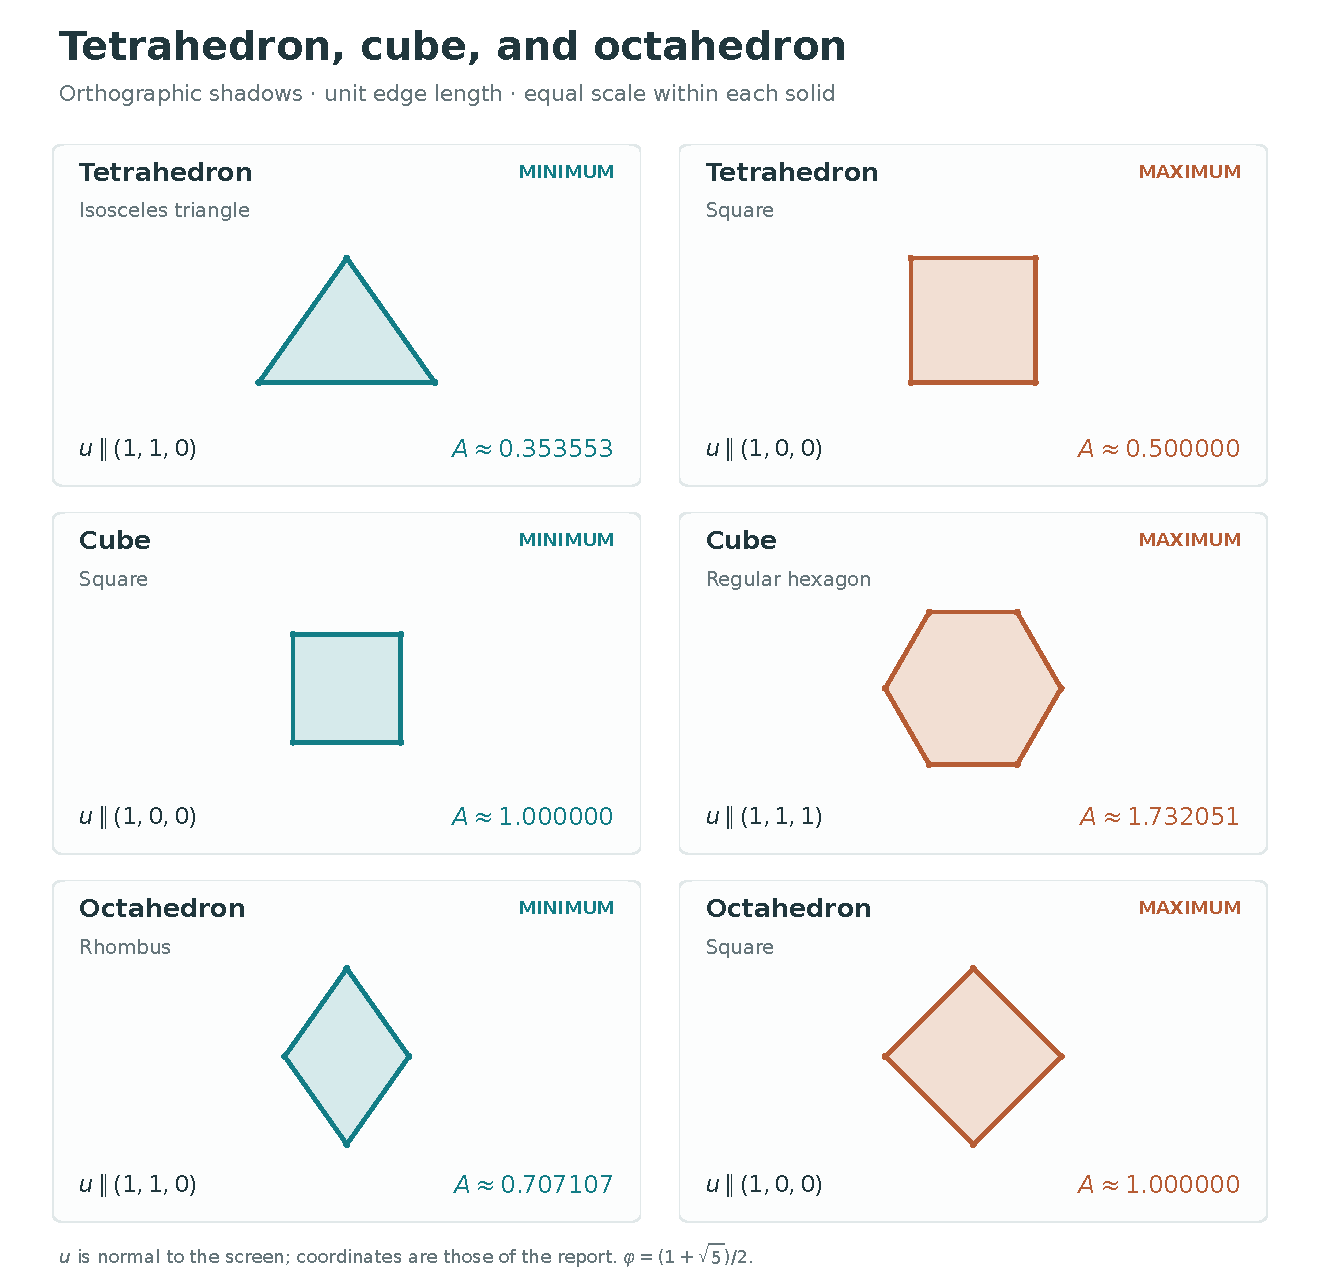
\includegraphics[width=\textwidth,height=.85\textheight,keepaspectratio]{figures/simple_shadows.pdf}
\end{center}
\small The two images within each row use the same scale. Every solid has unit edge length. Teal indicates a minimum and rust a maximum. Viewing vectors are normal to the screen and use the coordinate models of Section~\ref{sec:geometry}.

\clearpage\normalsize
\section*{Extremal shadow gallery: the golden-ratio solids}
\begin{center}
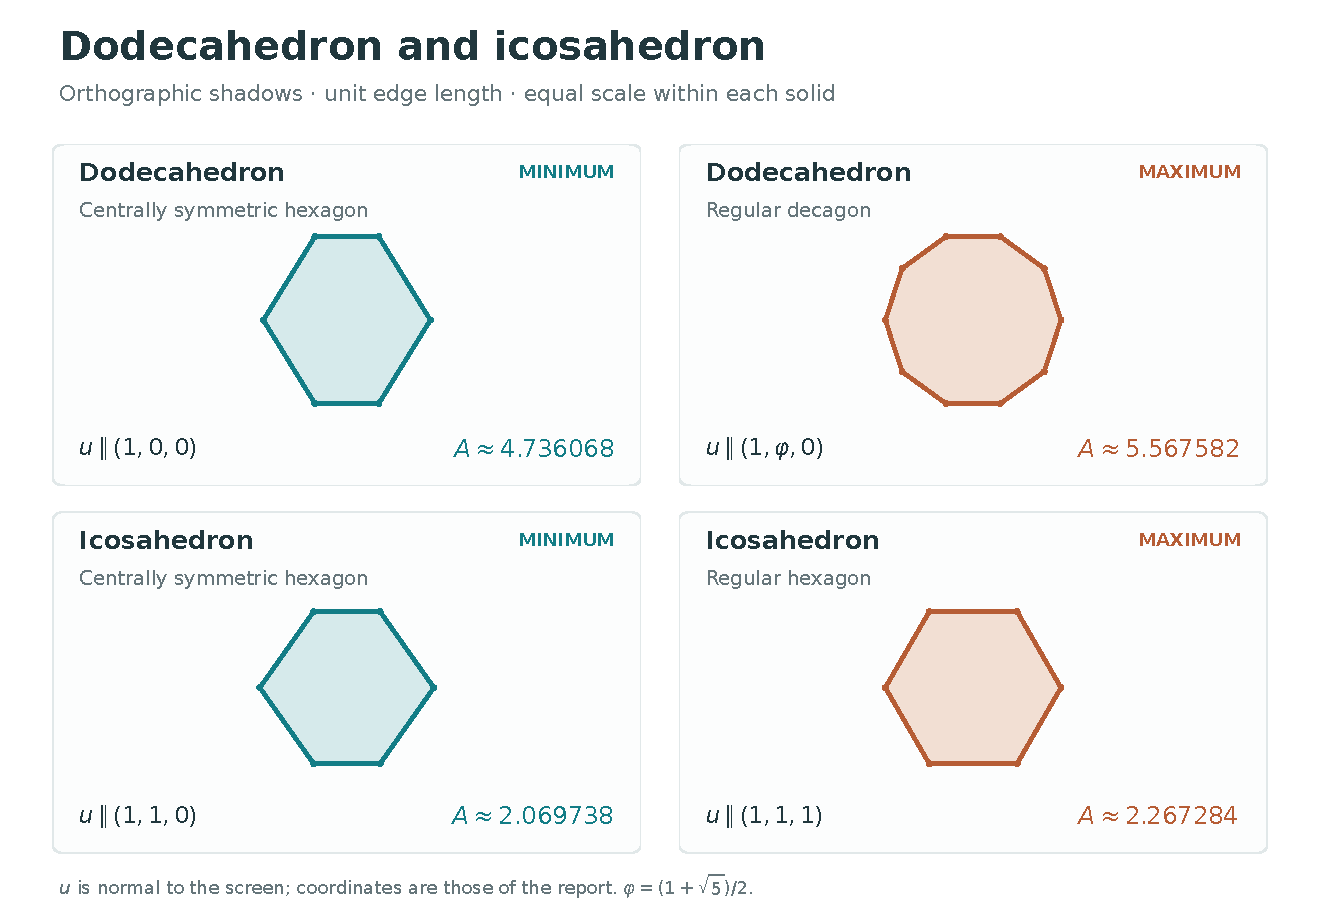
\includegraphics[width=\textwidth,height=.78\textheight,keepaspectratio]{figures/golden_shadows.pdf}
\end{center}
\small The icosahedron's minimum uses the direction $(1,1,0)$ in its stated coordinates, with two faces sharing a vertex but no edge seen edge-on. Its maximum is the regular hexagonal face-normal view. The diagrams are orthographic shadows, not planar sections.
\end{document}
